\section{Resolução do Desafio}

\begin{minipage}{\linewidth}
  \centering
  \begin{minipage}{0.45\linewidth}
    Dado o circuito da \textbf{Figura \ref{fig:CircuitoDesafioResolucao}}, identificar:
    \begin{itemize}
      \item Os componentes presentes;
      \item As funções de cada componente;
      \item A configuração de ligação dos componentes: série ou paralelo.
    \end{itemize}
  \end{minipage}
  \hspace{0.05\linewidth}
  \begin{minipage}{0.45\linewidth}
    \begin{figure}[H]
      \centering
      \caption{Circuito elétrico}
      \label{fig:CircuitoDesafioResolucao}
      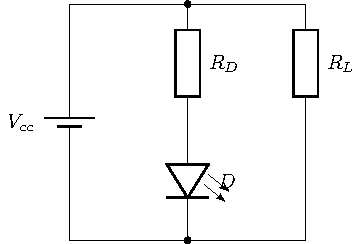
\includegraphics[scale=1.0]{fig-circuitoDesafio}
%
%      {\small Fonte: Próprio autor.}
    \end{figure}
  \end{minipage}
\end{minipage}



\subsection{Resolução}

\begin{itemize}
  \item Componente: função;
  \begin{itemize}
    \item $V_{CC}$: Fonte de Alimentação do circuito;
    \item $R_D$: Resistor limitador de corrente para o LED $D$;
    \item $D$: Dispositivo de sinalização luminosa, LED;
    \item $R_L$: Dispositivo de aquecimento, resistor de carga.
  \end{itemize}

  \item A configuração de ligação dos componentes: série ou paralelo.
  \begin{itemize}
    \item Fonte(gerador) está em paralelo com o restante do circuito, consumidor.
    \item $R_D$ está em série com o LED $D$.
    \item $R_L$ está em paralelo com o ramo inteiro do $R_D$ e $D$ e também em paralelo com a fonte.
    Note que $R_L$ não está em paralelo individualmente com $R_D$ e nem com o $D$, mas sim com os dois componentes associados.
  \end{itemize}
\end{itemize}
